\section{Additional Explanations}
\subsection{Converting Trace to Vector Clock representation}

\begin{figure}[h]
     \centering
     \subfloat[][Trace without Annotation]{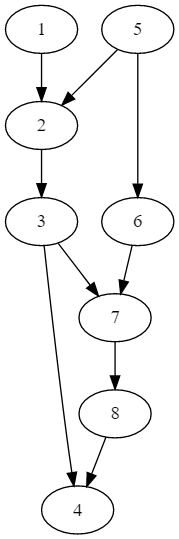
\includegraphics[scale=0.5]{figs/trace_without_ann.png}\label{trace_without_ann}}
     \subfloat[][Trace with Annotation]{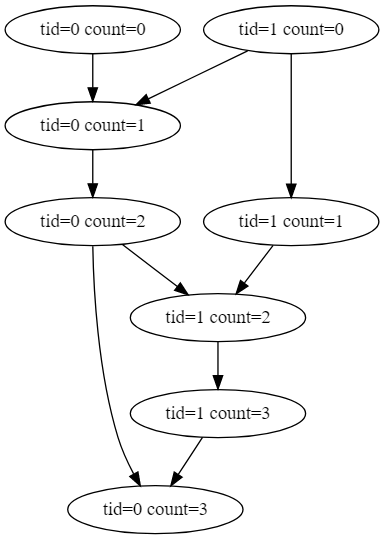
\includegraphics[scale=0.5]
{figs/trace_with_ann.png}
\label{trace_with_ann}}
     \caption{Trace representation in Graphviz}
\end{figure}

Mazurkiewicz trace~\citep{mazurkiewicz1986trace} is an  equivalence class representation of a multithreaded program execution. 
Figure~\ref{trace_without_ann} depicts an execution trace of a multithreaded program with two threads. 
Figure~\ref{trace_with_ann} is the annotated equivalence  of the trace in figure~\ref{trace_without_ann}. 
The trace file used by the IRS user space implementation is implemented using graphviz library. 
The figures~\ref{trace_without_ann} and \ref{trace_with_ann} are PNG representations of the graphviz file used as traces for a multithreaded program. 
From the trace file representation, we can assume that the multithreaded program uses two threads. 
There are in total of 4 shared memory events per thread considered in the above trace. 
However, there are only three memory constraints exhibited in the above trace. 
The three memory constraints converge at the nodes 2,7 and 4 respectively in the figure~\ref{trace_without_ann}. 
Memory constraints are mainly the shared memory access dependencies between the threads. 
From the above trace, we can observe that there are 3 points of these dependencies among two threads. 

\begin{figure}[h]
\centering
\begin{tabular}{c}
\begin{lstlisting}
{
  (1,[1:1]),
  (2,[3:2]),
  (1,[3:4])
}
\end{lstlisting}
\end{tabular}
\caption{Vector clock representation of the trace}
\label{vec_clk_repr}
\end{figure}


In this thesis, we move the scheduling decisions to kernel space. 
The prototypes highlighted in chapter~\ref{approach_ch} address various scheduler designs in kernel space. 
The scheduler requires the trace file as one of the inputs, as depicted in figure~\ref{design_overview}. 
However, as described in chapter~\ref{approach_ch} there are few design challenges in migrating the trace file represented as graphviz to kernel space. 
To overcome the challenge we have used an alternative representation of the trace to realize the scheduling constraints in kernel space scheduler module. 
Vector clock representation is the alternative representation considered for the above problem. 
Figure~\ref{vec_clk_datatype} is the data-type realized in kernel space to store the vector clock representation. 
The trace representation depicted in figure~\ref{trace_without_ann} would be transformed into a vector clock representation(vector clock representation is actually a string representation). 

\begin{figure}[h]
\centering
\begin{tabular}{c}
\begin{lstlisting}
struct vec_clk{
   int clocks[THREAD_COUNT];
};
\end{lstlisting}
\end{tabular}
\caption{Vector clock data type in kernel space}
\label{vec_clk_datatype}
\end{figure}

\begin{figure}[h]
\centering
\begin{tabular}{c}
\begin{lstlisting}
struct trace_node{
   thread_id_t thread_id;
   vec_clk clk;
   int valid;
};
\end{lstlisting}
\end{tabular}
\caption{Trace Node Representation in kernel space}
\label{trace_node_datatype}
\end{figure}



In our thesis, we have the thread ids in range from 1 to N. 
Therefore, in the above example thread id 0 is now 1 and thread id 1 is 2. 
Figure~\ref{vec_clk_repr} represents the vector representation of the trace depicted in figure~\ref{trace_without_ann}. 
This string is generated manually and passed as an input of the trace\_reg proc file. 
Let us disassemble the string to get an understanding of how it is parsed in kernel space. 
The curly braces determine the start and end of a given trace file. 
The values within the parenthesis focuses on a single node in the graph which emphasises on a memory constraint for a certain thread. 
In our vector representation, we have $(1,[1:1])$ as the first memory constraint. 
The first value after the opening parenthesis is the thread id, in regard to the first node it is thread id 1. 
The values within the square brackets are the number of events completed by each thread. 
These values within the square brackets are separated by a colon symbol. 
In case of the first node, we have thread id waiting for the completion of an event each in threads with ids 1 and 2. 
The thread id 1 is only allowed to progress if the vector clock state is equal to or surpassed the above mentioned vectored state. 
The string is parsed in kernel space when passed as a parameter to the custom proc file trace\_reg. 
Figure~\ref{trace_node_datatype} is the data type to which the parsed string is stored in kernel space. 

\subsection{Semaphores}

Semaphore is a variable or abstract data type used to control access to a common resource by multiple processes in a concurrent system~\citep{dijkstra1968cooperating}\citep{dijkstra1968structure}. 
Semaphores are useful programming abstractions used to prevent race conditions in concurrent programs. 
There are two types of semaphores - binary semaphore and counting semaphores. 
Counting semaphores are semaphores which allow an arbitrary resource count. 
Whereas binary semaphores are restricted to only two values 0 and 1. 
Binary semaphores are generally used to implement locks. 
In Linux kernel semaphores are realized under $linux/semaphore.h$. 
Semaphores are defined using the C struct $struct\ semaphore$. 
$sema\_init()$ is used to initialize a semaphore. 
In semaphores, we have up and down operations which deal with the increment and decrement of the value stored in the semaphore. 
In semaphores when the value of the semaphore is 0 and if a down operation is performed, the semaphore would block the thread who called the down operation. 
The thread is only resumed until an up operation of semaphore is performed by some other thread. 
In Linux, we have different types of down operations and one up operation. 
$down()$  is the conventional down operation which block the task until the semaphore value is retained to a positive value. 
$down\_interruptible()$ is similar to $down()$ but can be   unblock the operation by triggering an interrupt from the user space. 
$down\_try\_lock()$ is another implementation of down operation in Linux. 
It uses a busy waiting design to constantly check if the  value is positive or not, and it is an interruptible design. 
Based on the performance requirement and design we use a suitable down operation. 
In this thesis, considering the debugging purposes we have used $down\_interruptible()$ as the down operation on the semaphore. 
In this thesis, we have used an array of binary semaphores, where each semaphore is meant for each thread used in the multithreaded program. 
The semaphore design is mainly used in Prototypes 1,2 and 5 designs used in this thesis. 
Listing~\ref{sample_semaphore} provides a sample adaptation of semaphores in Linux kernel. 
The function $some\_dec\_operation()$ is blocked on $down\_interruptible()$ call if value of $sem$ is still 0 before the call. 
In $some\_inc\_operation()$ function we perform an $up$ operation on $sem$ thus, allowing any thread blocked on $sem$ to resume. 
\begin{lstlisting}[mathescape=true,style=customc,caption={Writing a sample Linux kernel program with semaphores},label={sample_semaphore}]
struct semaphore sem;
//kernel module initialization method
module_init() {
	...
	sema_init(&sem, 0);
}
...
void some_dec_operation() {
	...
	down_interruptible(&sem);	
	...
}
void some_inc_operation() {
	...
	up(&sem);
	...
}

\end{lstlisting}

 


\subsection{Scheduler APIs}

Scheduler APIs are a programming abstraction provided by the Linux Kernel for interacting with the OS scheduler. 
The scheduler APIs are located inside the headerfile $linux/sched.h$. 
They provide a lot functions to interact with the scheduler. 
Some of them include the setting of the scheduler with a specific scheduling policy, setting CPU affinity of certain kernel level task, etc. 
We are more interested in the APIs which deal with the wait queue and running queue of the OS scheduler. 
All threads or processes from user space are realized as tasks in kernel space. 
For every kernel level task there is a $task\ struct$ associated with it. 
To know more about $task\ struct$ please check the headerfile $linux/sched.h$. 
In this thesis, we obtain the task struct associated with the thread and push the task to the wait queue when we need to block the thread associated with the task. 
The task would be later resumed by some other task by invoking another scheduler API. 
For the blocking a task, we have a combination of two methods. 
Initially, we call $set\_current\_task(TASK\_INTERRUPTIBLE)$ which sets the task state of the calling task to wait state(TASK\_INTERRUPTIBLE means it could be revived on some interrupts from the machine). 
After this step, we call the method $schedule()$ which would relinquish the thread's control over the CPU. 
In short, with these two steps you have pushed the thread to wait queue of the OS scheduler. 
If the blocked thread needs to be revived, another task would invoke the method $wake\_up\_process(sleeping\_task)$. 
The task which invokes $wake\_up\_process()$ needs to have the $task\ struct$ of the blocked thread. 
Prototypes 3,4 and 6 mentioned in this thesis use this technique for blocking and unblocking the threads. 
 

\subsection{False Sharing}

False sharing is a performance-degrading usage pattern which can arise in distributed systems~\citep{torrellas1994false}. 
This problem mainly occurs in SMP(Symmetric Multiprocessor) systems where each processor has a local cache. 
It occurs when threads on different processors modify different memory locations that reside on the same cache line. 
Since these modifications made to the memory locations are not the same locations on a global viewpoint, the cache invalidation occurs because of these modifications. 
Thus, leading to a false sharing of the memory locations among threads. 
Programming constructs such as C-structs are more susceptible to false sharing problems~\citep{torrellas1994false}. 
The vector clock data type depicted in figure~\ref{vec_clk_datatype} is more susceptible to false sharing problem when the entire array is mapped under a single cache line. 
False sharing degrades the performance of the distributed application. 
In our thesis, we use the vector clock representation which uses a C struct representation. 
Since the C structs are susceptible to false sharing, our vector clock data type is susceptible as well. 
In chapter~\ref{eval_ch}, we perform a scaling of processor cores and we can observe in those evaluations the prototypes depicted in this thesis suffer from scalability problems. 
False sharing could be regarded as one of these problems. 
One way to fix the problem would be removing the C-struct representation and represent the vector clock datatype as normal array of integers.
 
\section{Building Prototypes}

All prototypes used in this thesis follow the same folder structure and also the operation of building them. 
Inside each prototype, we have an $include$, $scheduler$ and $Std\_Thread\_Impl$. 
$scheduler$ folder deals with the business logic of the prototype which the scheduler module and processing of the trace. 
$include$ folder contains three headerfiles - $common.h$, $kernel\_space.h$ and $user\_space.h$. 
The headers inside $include$ are mainly common headers used by the designs implemented in their respective scope(implementation scope means implementation is done either in kernel space or user space). 
$Std\_Thread\_Impl$ contains the benchmarking programs used for the evaluation of the prototypes. 

\subsection*{Loading and Unloading the Prototype}

Before we load the prototype to kernel space, we need to know the number of threads used in the multithreaded program. 
Currently, all the prototypes have the $THREAD\_COUNT$ parameter as statically defined. 
You have to modify the macro entry $THREAD\_COUNT$ inside the headerfile $common.h$ with the number of threads you have in your multithreaded program. 
Once that step is complete, you can load the kernel module by running the makefile located in the root directory of the prototype with target load. 
The command $make\ load$ will compile and load the prototype to kernel space with the number of threads you have indicated in the $common.h$ headerfile. 
The command $make\ unload$ will remove the module from the kernel space and clean up the module versions from your machine. 

\subsection*{Invoking Prototype related functions from a Multithreaded Program}

We have five main functions which are defined in the headerfile $user\_space.h$. 
These functions are $BeforeMA()$, $AfterMA()$, $initialize\_trace()$, $reset\_clock()$ and $thread\_reg()$. 
Currently, these prototypes are not integrated with LLVM therefore, methods such as $BeforeMA()$ and $AfterMA()$ needs to be invoked at the point of every shared memory event of the threads manually. 
But this functionality could be modified once integrated with LLVM. 
These two function expect the thread id which is value in the range of 1 to N. 
$initialize\_trace()$ is the first method which needs to be invoked from the multithreaded program. 
The method needs to be called before the creation of the threads and it expects a vector clock representation similar to the one shown in figure~\ref{vec_clk_repr}, but without newline and white space characters. 
$thread\_reg()$ needs to be called first within the thread function for registering the thread and it expects a thread id similar to $BeforeMA()$. 
$reset\_clock()$ is the final method which needs to be used with the multithreaded program. 
This method needs to be used once all the threads have completed their execution. 
The program needs to be run in superuser mode because the created IOCTL device requires root permissions access. 
The multithreaded should only be compiled and executed until the prototype module is loaded successfully.  




